\documentclass[]{book}
\usepackage{lmodern}
\usepackage{amssymb,amsmath}
\usepackage{ifxetex,ifluatex}
\usepackage{fixltx2e} % provides \textsubscript
\ifnum 0\ifxetex 1\fi\ifluatex 1\fi=0 % if pdftex
  \usepackage[T1]{fontenc}
  \usepackage[utf8]{inputenc}
\else % if luatex or xelatex
  \ifxetex
    \usepackage{mathspec}
  \else
    \usepackage{fontspec}
  \fi
  \defaultfontfeatures{Ligatures=TeX,Scale=MatchLowercase}
\fi
% use upquote if available, for straight quotes in verbatim environments
\IfFileExists{upquote.sty}{\usepackage{upquote}}{}
% use microtype if available
\IfFileExists{microtype.sty}{%
\usepackage{microtype}
\UseMicrotypeSet[protrusion]{basicmath} % disable protrusion for tt fonts
}{}
\usepackage{hyperref}
\hypersetup{unicode=true,
            pdftitle={Hurricane Analysis and Visulization Using R},
            pdfauthor={Romane Goldmuntz, Vy Tran, and Jianqiong Zhan},
            pdfborder={0 0 0},
            breaklinks=true}
\urlstyle{same}  % don't use monospace font for urls
\usepackage{natbib}
\bibliographystyle{apalike}
\usepackage{color}
\usepackage{fancyvrb}
\newcommand{\VerbBar}{|}
\newcommand{\VERB}{\Verb[commandchars=\\\{\}]}
\DefineVerbatimEnvironment{Highlighting}{Verbatim}{commandchars=\\\{\}}
% Add ',fontsize=\small' for more characters per line
\usepackage{framed}
\definecolor{shadecolor}{RGB}{248,248,248}
\newenvironment{Shaded}{\begin{snugshade}}{\end{snugshade}}
\newcommand{\AlertTok}[1]{\textcolor[rgb]{0.94,0.16,0.16}{#1}}
\newcommand{\AnnotationTok}[1]{\textcolor[rgb]{0.56,0.35,0.01}{\textbf{\textit{#1}}}}
\newcommand{\AttributeTok}[1]{\textcolor[rgb]{0.77,0.63,0.00}{#1}}
\newcommand{\BaseNTok}[1]{\textcolor[rgb]{0.00,0.00,0.81}{#1}}
\newcommand{\BuiltInTok}[1]{#1}
\newcommand{\CharTok}[1]{\textcolor[rgb]{0.31,0.60,0.02}{#1}}
\newcommand{\CommentTok}[1]{\textcolor[rgb]{0.56,0.35,0.01}{\textit{#1}}}
\newcommand{\CommentVarTok}[1]{\textcolor[rgb]{0.56,0.35,0.01}{\textbf{\textit{#1}}}}
\newcommand{\ConstantTok}[1]{\textcolor[rgb]{0.00,0.00,0.00}{#1}}
\newcommand{\ControlFlowTok}[1]{\textcolor[rgb]{0.13,0.29,0.53}{\textbf{#1}}}
\newcommand{\DataTypeTok}[1]{\textcolor[rgb]{0.13,0.29,0.53}{#1}}
\newcommand{\DecValTok}[1]{\textcolor[rgb]{0.00,0.00,0.81}{#1}}
\newcommand{\DocumentationTok}[1]{\textcolor[rgb]{0.56,0.35,0.01}{\textbf{\textit{#1}}}}
\newcommand{\ErrorTok}[1]{\textcolor[rgb]{0.64,0.00,0.00}{\textbf{#1}}}
\newcommand{\ExtensionTok}[1]{#1}
\newcommand{\FloatTok}[1]{\textcolor[rgb]{0.00,0.00,0.81}{#1}}
\newcommand{\FunctionTok}[1]{\textcolor[rgb]{0.00,0.00,0.00}{#1}}
\newcommand{\ImportTok}[1]{#1}
\newcommand{\InformationTok}[1]{\textcolor[rgb]{0.56,0.35,0.01}{\textbf{\textit{#1}}}}
\newcommand{\KeywordTok}[1]{\textcolor[rgb]{0.13,0.29,0.53}{\textbf{#1}}}
\newcommand{\NormalTok}[1]{#1}
\newcommand{\OperatorTok}[1]{\textcolor[rgb]{0.81,0.36,0.00}{\textbf{#1}}}
\newcommand{\OtherTok}[1]{\textcolor[rgb]{0.56,0.35,0.01}{#1}}
\newcommand{\PreprocessorTok}[1]{\textcolor[rgb]{0.56,0.35,0.01}{\textit{#1}}}
\newcommand{\RegionMarkerTok}[1]{#1}
\newcommand{\SpecialCharTok}[1]{\textcolor[rgb]{0.00,0.00,0.00}{#1}}
\newcommand{\SpecialStringTok}[1]{\textcolor[rgb]{0.31,0.60,0.02}{#1}}
\newcommand{\StringTok}[1]{\textcolor[rgb]{0.31,0.60,0.02}{#1}}
\newcommand{\VariableTok}[1]{\textcolor[rgb]{0.00,0.00,0.00}{#1}}
\newcommand{\VerbatimStringTok}[1]{\textcolor[rgb]{0.31,0.60,0.02}{#1}}
\newcommand{\WarningTok}[1]{\textcolor[rgb]{0.56,0.35,0.01}{\textbf{\textit{#1}}}}
\usepackage{longtable,booktabs}
\usepackage{graphicx,grffile}
\makeatletter
\def\maxwidth{\ifdim\Gin@nat@width>\linewidth\linewidth\else\Gin@nat@width\fi}
\def\maxheight{\ifdim\Gin@nat@height>\textheight\textheight\else\Gin@nat@height\fi}
\makeatother
% Scale images if necessary, so that they will not overflow the page
% margins by default, and it is still possible to overwrite the defaults
% using explicit options in \includegraphics[width, height, ...]{}
\setkeys{Gin}{width=\maxwidth,height=\maxheight,keepaspectratio}
\IfFileExists{parskip.sty}{%
\usepackage{parskip}
}{% else
\setlength{\parindent}{0pt}
\setlength{\parskip}{6pt plus 2pt minus 1pt}
}
\setlength{\emergencystretch}{3em}  % prevent overfull lines
\providecommand{\tightlist}{%
  \setlength{\itemsep}{0pt}\setlength{\parskip}{0pt}}
\setcounter{secnumdepth}{5}
% Redefines (sub)paragraphs to behave more like sections
\ifx\paragraph\undefined\else
\let\oldparagraph\paragraph
\renewcommand{\paragraph}[1]{\oldparagraph{#1}\mbox{}}
\fi
\ifx\subparagraph\undefined\else
\let\oldsubparagraph\subparagraph
\renewcommand{\subparagraph}[1]{\oldsubparagraph{#1}\mbox{}}
\fi

%%% Use protect on footnotes to avoid problems with footnotes in titles
\let\rmarkdownfootnote\footnote%
\def\footnote{\protect\rmarkdownfootnote}

%%% Change title format to be more compact
\usepackage{titling}

% Create subtitle command for use in maketitle
\providecommand{\subtitle}[1]{
  \posttitle{
    \begin{center}\large#1\end{center}
    }
}

\setlength{\droptitle}{-2em}

  \title{Hurricane Analysis and Visulization Using R}
    \pretitle{\vspace{\droptitle}\centering\huge}
  \posttitle{\par}
    \author{Romane Goldmuntz, Vy Tran, and Jianqiong Zhan}
    \preauthor{\centering\large\emph}
  \postauthor{\par}
      \predate{\centering\large\emph}
  \postdate{\par}
    \date{2019-11-07}

\usepackage{booktabs}
\usepackage{amsthm}
\makeatletter
\def\thm@space@setup{%
  \thm@preskip=8pt plus 2pt minus 4pt
  \thm@postskip=\thm@preskip
}
\makeatother

\begin{document}
\maketitle

{
\setcounter{tocdepth}{1}
\tableofcontents
}
\hypertarget{preface}{%
\chapter{Preface}\label{preface}}

This is a class project written in \textbf{Markdown}. We are still working on it.

We are using the \textbf{bookdown} package \citep{R-bookdown} in this project, which was built on top of R Markdown and \textbf{knitr} \citep{xie2015}.

\hypertarget{intro}{%
\chapter{Introduction}\label{intro}}

As coastal shoreline counties create about 40\% of the United States's jobs and account for 46\% of its GDP, hurricanes have a trumendous impact on the country's economy.

They are considered as one of the costliest natural disasters in the world : they currently cost the government over \$28 billion each year, and that amount is expected to increase to over \$39 billion a year due to the increased development of the U.S. coastlines and the global warming. The latter will indeed increase the proportion of cyclones of category 4 and 5, which lead to the most damages and therefore higher costs \citep{Amadeo2019}.

Besides the government, several industries are heavily impacted by hurricanes, including the insurance industry. For example, according to Bloomberg, hurricane Dorian caused the insurance industry losses of up \$25 billion, making it the most expensive natural disaster for the industry since 2017's Hurricane Maria \citep{DSouza2019}.

Reference a figure by its code chunk label with the \texttt{fig:} prefix, e.g., see Figure \ref{fig:nice-fig}.

\begin{Shaded}
\begin{Highlighting}[]
\KeywordTok{library}\NormalTok{(rvest)}
\KeywordTok{library}\NormalTok{(dplyr)}
\KeywordTok{library}\NormalTok{(robotstxt)}
\KeywordTok{library}\NormalTok{(ggplot2)}
\NormalTok{url <-}\StringTok{ "https://en.wikipedia.org/wiki/List_of_costliest_Atlantic_hurricanes"}
\CommentTok{#paths_allowed(url)}

\NormalTok{df<-}\KeywordTok{as.data.frame}\NormalTok{(}\KeywordTok{read_html}\NormalTok{(url) }\OperatorTok\StringTok{ }\KeywordTok{html_table}\NormalTok{(}\DataTypeTok{fill =} \OtherTok{TRUE}\NormalTok{))}

\NormalTok{df_clean <-}\StringTok{ }\NormalTok{df }\OperatorTok\StringTok{ }\KeywordTok{mutate}\NormalTok{(}\DataTypeTok{Nominal_Damage =} \KeywordTok{as.factor}\NormalTok{(}\KeywordTok{gsub}\NormalTok{(}\StringTok{"[$><]"}\NormalTok{, }\StringTok{""}\NormalTok{,Nominal.damage.Billions.USD.)))}\OperatorTok
\StringTok{  }\KeywordTok{select}\NormalTok{(Name, Season, Storm.classificationat.peak.intensity,Nominal_Damage) }\OperatorTok\StringTok{ }\KeywordTok{rename}\NormalTok{(}\DataTypeTok{Classification =}\NormalTok{ Storm.classificationat.peak.intensity)}
\NormalTok{df_clean}\OperatorTok{$}\NormalTok{Season<-}\KeywordTok{as.factor}\NormalTok{(df_clean}\OperatorTok{$}\NormalTok{Season)}
\NormalTok{as.numeric.factor <-}\StringTok{ }\ControlFlowTok{function}\NormalTok{(x) \{}\KeywordTok{as.numeric}\NormalTok{(}\KeywordTok{levels}\NormalTok{(x))[x]\}}
\NormalTok{df_clean[}\DecValTok{4}\NormalTok{]<-}\KeywordTok{lapply}\NormalTok{(df_clean[}\DecValTok{4}\NormalTok{],as.numeric.factor)}
\NormalTok{df_clean[}\DecValTok{2}\NormalTok{]<-}\KeywordTok{lapply}\NormalTok{(df_clean[}\DecValTok{2}\NormalTok{],as.numeric.factor)}
\NormalTok{df_clean <-}\StringTok{ }\NormalTok{df_clean }\OperatorTok\StringTok{ }\KeywordTok{arrange}\NormalTok{(}\KeywordTok{desc}\NormalTok{(Season)) }\OperatorTok\StringTok{ }\KeywordTok{top_n}\NormalTok{(}\DecValTok{6}\NormalTok{)}
\KeywordTok{ggplot}\NormalTok{(df_clean,}\KeywordTok{aes}\NormalTok{(}\DataTypeTok{x=}\NormalTok{Name, }\DataTypeTok{y=}\NormalTok{ Nominal_Damage)) }\OperatorTok{+}\StringTok{ }\KeywordTok{geom_bar}\NormalTok{(}\DataTypeTok{position =} \StringTok{"dodge"}\NormalTok{, }\DataTypeTok{stat =} \StringTok{"identity"}\NormalTok{) }\OperatorTok{+}\StringTok{ }\KeywordTok{coord_flip}\NormalTok{() }\OperatorTok{+}\StringTok{ }\KeywordTok{xlab}\NormalTok{(}\StringTok{"Hurricane"}\NormalTok{) }\OperatorTok{+}\StringTok{ }\KeywordTok{ylab}\NormalTok{(}\StringTok{"Damage (in Billion Dollars)"}\NormalTok{) }\OperatorTok{+}\StringTok{ }\KeywordTok{ggtitle}\NormalTok{(}\StringTok{"Cost of Damage by Six Most Recent Hurricanes"}\NormalTok{) }\OperatorTok{+}\StringTok{ }\KeywordTok{theme_classic}\NormalTok{()}
\end{Highlighting}
\end{Shaded}

\begin{figure}

{\centering 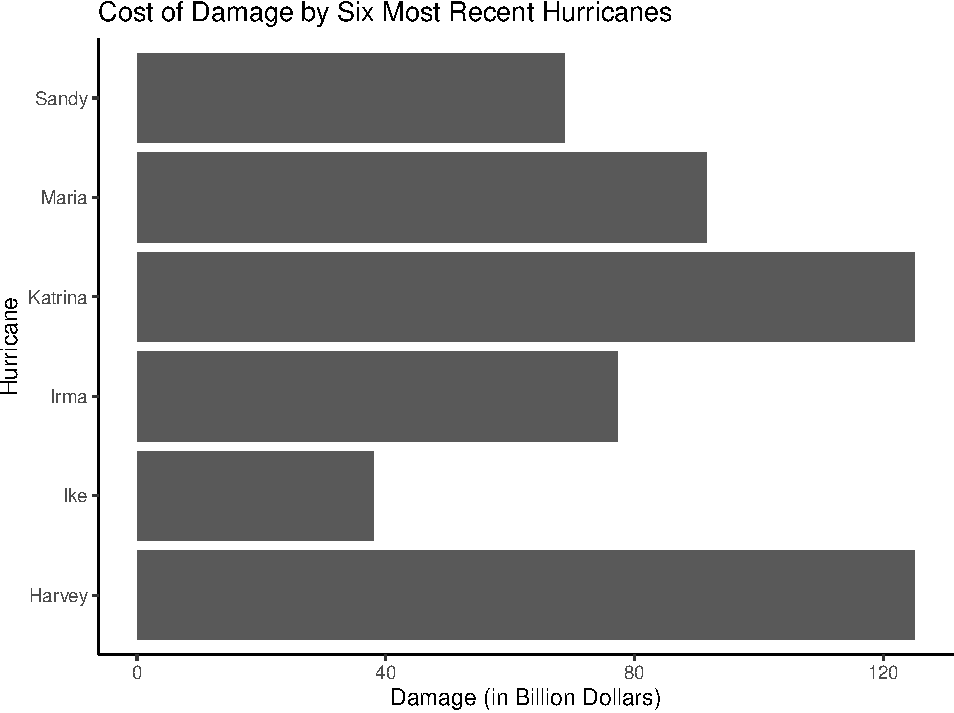
\includegraphics[width=0.8\linewidth]{edav-final-project_files/figure-latex/nice-fig-1} 

}

\caption{Here is a nice figure!}\label{fig:nice-fig}
\end{figure}

In addition, hurricane tracking data can provide Federal Emergency Management Agency (FEMA), local emergency managers, and first responders the information they need to be able to send out appropriate responses and help to the citizens at the affected areas \citep{Newtools4H2019}.

For those reasons, hurricanes data is very interesting to analyze and will constitute the topic of this Exploratory Data Analysis and Vizualisation final project.

\hypertarget{methods}{%
\chapter{Methods}\label{methods}}

\hypertarget{data-sources}{%
\section{Data sources}\label{data-sources}}

(We describe our data sources, our methods in this chapter)

Storm tracks data can be downloaded from \href{https://www.nhc.noaa.gov/data/\#hurdat}{National Hurricane Center and Central Pacific Hurricane Center}. The data using in the project is known as Atlantic hurricane database (\href{https://www.nhc.noaa.gov/data/hurdat/hurdat2-format-atlantic.pdf}{HURDAT2}) 1851-2018 (\href{https://www.nhc.noaa.gov/data/hurdat/hurdat2-1851-2018-051019.txt}{5.9MB download}). The data has a comma-delimited, text format with six-hourly information on the location, maximum winds, central pressure, and (beginning in 2004) size of all known tropical cyclones and subtropical cyclones.

\hypertarget{data-transformat}{%
\section{Data transformat}\label{data-transformat}}

(Describe the process of getting the data into a form in which you could work with it in R.)

** load libraries **

\begin{Shaded}
\begin{Highlighting}[]
\KeywordTok{library}\NormalTok{(tidyverse)}
\KeywordTok{library}\NormalTok{(stringr)}
\CommentTok{# Read in data set}
\CommentTok{#dfile <- read_lines("https://www.nhc.noaa.gov/data/hurdat/hurdat2-1851-2018-051019.txt")}
\NormalTok{dfile<-}\StringTok{ "data/hurdat2-1851-2018-051019.txt"}
\NormalTok{hurdat2_in <-}\StringTok{ }\KeywordTok{read_lines}\NormalTok{(dfile)}
\end{Highlighting}
\end{Shaded}

The dataset is a combination of serveral subsets. Eeach subset is for a storm track record which incluedes header information and values.

\emph{For instance, the header has the following format:}

AL162018, OSCAR, 36,
* AL -- Basin -- Atlantic
* 16 -- ATCF cyclone number for that year
* 2018 -- Year
* OSCAR -- Name, if available, or else ``UNNAMED''
* 36 -- Number of best track entries -- rows -- to follow

\emph{The header is followed by data, which has the following format:}

20181026, 1800, , SS, 25.4N, 45.3W, 35, 1006, 80, 80, 0, 0, 0, 0, 0, 0, 0, 0, 0, 0,

\begin{itemize}
\tightlist
\item
  2018 -- Year
\item
  10 -- Month
\item
  26 -- Day
\item
  09 -- Hours in UTC (Universal Time Coordinate) 35 (Spaces 13-14, before 2nd comma) -- Minutes
  \ldots{}
\end{itemize}

\textbf{please refer \href{\%22https://www.nhc.noaa.gov/data/hurdat/hurdat2-format-atlantic.pdf\%22}{this file} for detail information.}

\begin{Shaded}
\begin{Highlighting}[]
\NormalTok{header_locations <-}\StringTok{ }\NormalTok{(}\DecValTok{1}\OperatorTok{:}\KeywordTok{length}\NormalTok{(hurdat2_in))[}\KeywordTok{str_count}\NormalTok{(hurdat2_in, }\StringTok{"}\CharTok{\textbackslash{}\textbackslash{}}\StringTok{,"}\NormalTok{) }\OperatorTok{==}\StringTok{ }\DecValTok{3}\NormalTok{]}
\NormalTok{header_df <-readr}\OperatorTok{::}\KeywordTok{read_csv}\NormalTok{(hurdat2_in[header_locations], }
                             \DataTypeTok{col_names =} \OtherTok{FALSE}\NormalTok{) }\OperatorTok\StringTok{ }
\StringTok{  }\NormalTok{dplyr}\OperatorTok{::}\KeywordTok{select}\NormalTok{(}\OperatorTok{-}\KeywordTok{c}\NormalTok{(}\StringTok{"X4"}\NormalTok{))}
\KeywordTok{names}\NormalTok{(header_df) <-}\StringTok{ }\KeywordTok{c}\NormalTok{(}\StringTok{"id"}\NormalTok{,}\StringTok{"name"}\NormalTok{,}\StringTok{"n_entries"}\NormalTok{)}
\end{Highlighting}
\end{Shaded}

\begin{Shaded}
\begin{Highlighting}[]
\CommentTok{# read hearder information}
\KeywordTok{library}\NormalTok{(stringr)}
\NormalTok{header_locations <-}\StringTok{ }\NormalTok{(}\DecValTok{1}\OperatorTok{:}\KeywordTok{length}\NormalTok{(hurdat2_in))[stringr}\OperatorTok{::}\KeywordTok{str_count}\NormalTok{(hurdat2_in, }\StringTok{"}\CharTok{\textbackslash{}\textbackslash{}}\StringTok{,"}\NormalTok{) }\OperatorTok{==}\StringTok{ }\DecValTok{3}\NormalTok{]}

\NormalTok{header_df <-}\StringTok{ }\NormalTok{readr}\OperatorTok{::}\KeywordTok{read_csv}\NormalTok{(hurdat2_in[header_locations], }
                             \DataTypeTok{col_names =} \OtherTok{FALSE}\NormalTok{) }\OperatorTok\StringTok{ }
\StringTok{  }\NormalTok{dplyr}\OperatorTok{::}\KeywordTok{select}\NormalTok{(}\OperatorTok{-}\KeywordTok{c}\NormalTok{(}\StringTok{"X4"}\NormalTok{))}

\KeywordTok{names}\NormalTok{(header_df) <-}\StringTok{ }\KeywordTok{c}\NormalTok{(}\StringTok{"id"}\NormalTok{,}\StringTok{"name"}\NormalTok{,}\StringTok{"n_entries"}\NormalTok{)}

\NormalTok{header_df <-}\StringTok{  }\NormalTok{header_df }\OperatorTok\StringTok{ }\KeywordTok{mutate}\NormalTok{(}\DataTypeTok{header_loc =} \KeywordTok{as.numeric}\NormalTok{(header_locations))}

\CommentTok{#tail(header_df)}
\end{Highlighting}
\end{Shaded}

\begin{Shaded}
\begin{Highlighting}[]
\CommentTok{# read data value}

\NormalTok{hurdat2_df <-}\StringTok{ }\KeywordTok{vector}\NormalTok{(}\StringTok{"list"}\NormalTok{, }\KeywordTok{nrow}\NormalTok{(header_df))}
\KeywordTok{names}\NormalTok{(hurdat2_df) <-}\StringTok{ }\NormalTok{header_df}\OperatorTok{$}\NormalTok{id}
\NormalTok{df_names <-}\StringTok{ }\KeywordTok{c}\NormalTok{(}
  \StringTok{"date"}\NormalTok{, }\StringTok{"time"}\NormalTok{, }\StringTok{"record_identifier"}\NormalTok{, }\StringTok{"status"}\NormalTok{, }\StringTok{"latitude"}\NormalTok{, }\StringTok{"longitude"}\NormalTok{, }\StringTok{"max_wind"}\NormalTok{, }\StringTok{"min_pressure"}\NormalTok{,}
  \StringTok{"extent_34_NE"}\NormalTok{, }\StringTok{"extent_34_SE"}\NormalTok{, }\StringTok{"extent_34_SW"}\NormalTok{, }\StringTok{"extent_34_NW"}\NormalTok{,}
  \StringTok{"extent_50_NE"}\NormalTok{, }\StringTok{"extent_50_SE"}\NormalTok{, }\StringTok{"extent_50_SW"}\NormalTok{, }\StringTok{"extent_50_NW"}\NormalTok{,}
  \StringTok{"extent_64_NE"}\NormalTok{, }\StringTok{"extent_64_SE"}\NormalTok{, }\StringTok{"extent_64_SW"}\NormalTok{, }\StringTok{"extent_64_NW"}\NormalTok{, }\StringTok{"nas"}
\NormalTok{)}

\CommentTok{#}
\ControlFlowTok{for}\NormalTok{ (i }\ControlFlowTok{in} \KeywordTok{seq_along}\NormalTok{(header_df}\OperatorTok{$}\NormalTok{id)) \{}
\NormalTok{  hurdat2_df[[i]] <-}\StringTok{ }\KeywordTok{read_csv}\NormalTok{(dfile,}
    \DataTypeTok{skip =}\NormalTok{ header_df}\OperatorTok{$}\NormalTok{header_loc[i],}
    \DataTypeTok{n_max =}\NormalTok{ header_df}\OperatorTok{$}\NormalTok{n_entries[i],}
    \DataTypeTok{col_names =}\NormalTok{ df_names,}
    \DataTypeTok{na =} \KeywordTok{c}\NormalTok{(}\StringTok{""}\NormalTok{, }\StringTok{"-99"}\NormalTok{, }\StringTok{"-999"}\NormalTok{),}
    \DataTypeTok{col_types =} \KeywordTok{list}\NormalTok{(}
      \DataTypeTok{time =} \KeywordTok{col_character}\NormalTok{(),}
      \DataTypeTok{min_pressure =} \KeywordTok{col_integer}\NormalTok{(),}
      \DataTypeTok{extent_34_NE =} \KeywordTok{col_integer}\NormalTok{(),}
      \DataTypeTok{extent_34_SE =} \KeywordTok{col_integer}\NormalTok{(),}
      \DataTypeTok{extent_34_SW =} \KeywordTok{col_integer}\NormalTok{(),}
      \DataTypeTok{extent_34_NW =} \KeywordTok{col_integer}\NormalTok{(),}
      \DataTypeTok{extent_50_NE =} \KeywordTok{col_integer}\NormalTok{(),}
      \DataTypeTok{extent_50_SE =} \KeywordTok{col_integer}\NormalTok{(),}
      \DataTypeTok{extent_50_SW =} \KeywordTok{col_integer}\NormalTok{(),}
      \DataTypeTok{extent_50_NW =} \KeywordTok{col_integer}\NormalTok{(),}
      \DataTypeTok{extent_64_NE =} \KeywordTok{col_integer}\NormalTok{(),}
      \DataTypeTok{extent_64_SE =} \KeywordTok{col_integer}\NormalTok{(),}
      \DataTypeTok{extent_64_SW =} \KeywordTok{col_integer}\NormalTok{(),}
      \DataTypeTok{extent_64_NW =} \KeywordTok{col_integer}\NormalTok{()}
\NormalTok{    )}
\NormalTok{  )}
\NormalTok{\}}
\end{Highlighting}
\end{Shaded}

\begin{Shaded}
\begin{Highlighting}[]
\CommentTok{#head(hurdat2_df)}
\end{Highlighting}
\end{Shaded}

\begin{Shaded}
\begin{Highlighting}[]
\CommentTok{# Combine and clean the data sets}
\KeywordTok{library}\NormalTok{(lubridate)}
\NormalTok{hurdat2 <-}\StringTok{ }
\StringTok{  }\NormalTok{hurdat2_df }\OperatorTok
\StringTok{  }\NormalTok{dplyr}\OperatorTok{::}\KeywordTok{bind_rows}\NormalTok{(}\DataTypeTok{.id =} \StringTok{"id"}\NormalTok{) }\OperatorTok
\StringTok{  }\NormalTok{dplyr}\OperatorTok{::}\KeywordTok{mutate}\NormalTok{(}
    \DataTypeTok{date =}\NormalTok{ lubridate}\OperatorTok{::}\KeywordTok{ymd}\NormalTok{(date),}
    \DataTypeTok{year =}\NormalTok{ lubridate}\OperatorTok{::}\KeywordTok{year}\NormalTok{(date),}
    \DataTypeTok{month =}\NormalTok{ lubridate}\OperatorTok{::}\KeywordTok{month}\NormalTok{(date),}
    \DataTypeTok{day =}\NormalTok{ lubridate}\OperatorTok{::}\KeywordTok{day}\NormalTok{(date),}
    \DataTypeTok{hour =} \KeywordTok{as.numeric}\NormalTok{(stringr}\OperatorTok{::}\KeywordTok{str_sub}\NormalTok{(time, }\DecValTok{1}\NormalTok{, }\DecValTok{2}\NormalTok{)),}
    \DataTypeTok{datetime =} \KeywordTok{as.Date}\NormalTok{(}\KeywordTok{ISOdate}\NormalTok{(year, month, day, hour, }\DataTypeTok{min =} \DecValTok{0}\NormalTok{, }\DataTypeTok{sec =} \DecValTok{0}\NormalTok{, }\DataTypeTok{tz =} \StringTok{"GMT"}\NormalTok{)),}
    \CommentTok{#lat_hemisphere = stringr::str_sub(latitude, -1),}
    \DataTypeTok{latitude =}\NormalTok{ dplyr}\OperatorTok{::}\KeywordTok{if_else}\NormalTok{(stringr}\OperatorTok{::}\KeywordTok{str_sub}\NormalTok{(latitude, }\DecValTok{-1}\NormalTok{) }\OperatorTok{==}\StringTok{ "N"}\NormalTok{,}
                              \KeywordTok{as.numeric}\NormalTok{(stringr}\OperatorTok{::}\KeywordTok{str_sub}\NormalTok{(latitude, }\DecValTok{1}\NormalTok{, }\DecValTok{-2}\NormalTok{))}\OperatorTok{*}\DecValTok{1}\NormalTok{, }
                              \KeywordTok{as.numeric}\NormalTok{(stringr}\OperatorTok{::}\KeywordTok{str_sub}\NormalTok{(latitude, }\DecValTok{1}\NormalTok{, }\DecValTok{-2}\NormalTok{))}\OperatorTok{*}\NormalTok{(}\OperatorTok{-}\DecValTok{1}\NormalTok{)),}
    \DataTypeTok{longitude =}\NormalTok{ dplyr}\OperatorTok{::}\KeywordTok{if_else}\NormalTok{(stringr}\OperatorTok{::}\KeywordTok{str_sub}\NormalTok{(longitude, }\DecValTok{-1}\NormalTok{) }\OperatorTok{==}\StringTok{ "E"}\NormalTok{,}
                              \KeywordTok{as.numeric}\NormalTok{(stringr}\OperatorTok{::}\KeywordTok{str_sub}\NormalTok{(longitude, }\DecValTok{1}\NormalTok{, }\DecValTok{-2}\NormalTok{))}\OperatorTok{*}\DecValTok{1}\NormalTok{, }
                              \KeywordTok{as.numeric}\NormalTok{(stringr}\OperatorTok{::}\KeywordTok{str_sub}\NormalTok{(longitude, }\DecValTok{1}\NormalTok{, }\DecValTok{-2}\NormalTok{))}\OperatorTok{*}\NormalTok{(}\OperatorTok{-}\DecValTok{1}\NormalTok{)),}
    \DataTypeTok{category =} \KeywordTok{cut}\NormalTok{(max_wind, }\CommentTok{# Saffir-Simpson Hurricane Wind Scale}
      \DataTypeTok{breaks =} \KeywordTok{c}\NormalTok{(}\DecValTok{0}\NormalTok{, }\DecValTok{34}\NormalTok{, }\DecValTok{64}\NormalTok{, }\DecValTok{83}\NormalTok{, }\DecValTok{96}\NormalTok{, }\DecValTok{113}\NormalTok{, }\DecValTok{137}\NormalTok{, }\DecValTok{500}\NormalTok{),}
      \DataTypeTok{labels =} \KeywordTok{c}\NormalTok{(}\OperatorTok{-}\DecValTok{1}\NormalTok{, }\DecValTok{0}\NormalTok{, }\DecValTok{1}\NormalTok{, }\DecValTok{2}\NormalTok{, }\DecValTok{3}\NormalTok{, }\DecValTok{4}\NormalTok{, }\DecValTok{5}\NormalTok{),}
      \DataTypeTok{include.lowest =} \OtherTok{TRUE}\NormalTok{, }\DataTypeTok{ordered =} \OtherTok{TRUE}
\NormalTok{    ),}
    \CommentTok{# wind = wind * 1.15078, # transforms knots to mph,}
    \DataTypeTok{TSradius1 =}\NormalTok{ extent_}\DecValTok{34}\NormalTok{_NE }\OperatorTok{+}\StringTok{ }\NormalTok{extent_}\DecValTok{34}\NormalTok{_SW,}
    \DataTypeTok{TSradius2 =}\NormalTok{ extent_}\DecValTok{34}\NormalTok{_NW }\OperatorTok{+}\StringTok{ }\NormalTok{extent_}\DecValTok{34}\NormalTok{_SE,}
    \DataTypeTok{ts_diameter =} \KeywordTok{pmax}\NormalTok{(TSradius1, TSradius2) }\OperatorTok{*}\StringTok{ }\FloatTok{1.15078}\NormalTok{, }\CommentTok{# to convert from nautical miles to miles # pmax: returns the parallel maxima and minima of the input values}
    \DataTypeTok{HUradius1 =}\NormalTok{ extent_}\DecValTok{64}\NormalTok{_NE }\OperatorTok{+}\StringTok{ }\NormalTok{extent_}\DecValTok{64}\NormalTok{_SW,}
    \DataTypeTok{HUradius2 =}\NormalTok{ extent_}\DecValTok{64}\NormalTok{_NW }\OperatorTok{+}\StringTok{ }\NormalTok{extent_}\DecValTok{64}\NormalTok{_SE,}
    \DataTypeTok{hu_diameter =} \KeywordTok{pmax}\NormalTok{(HUradius1, HUradius2) }\OperatorTok{*}\StringTok{ }\FloatTok{1.15078}\NormalTok{, }\CommentTok{# to convert from nautical miles to miles # pmax: returns the parallel maxima and minima of the input values}
    \DataTypeTok{status =} \KeywordTok{recode}\NormalTok{(status,}
                    \StringTok{"TD"}\NormalTok{ =}\StringTok{ "tropical depression"}\NormalTok{,}
                    \StringTok{"TS"}\NormalTok{ =}\StringTok{ "tropical storm"}\NormalTok{, }
                    \StringTok{"HU"}\NormalTok{ =}\StringTok{ "tropical hurricane"}\NormalTok{, }
                    \StringTok{"EX"}\NormalTok{ =}\StringTok{ "Extratropical cyclone"}\NormalTok{, }\CommentTok{##}
                    \StringTok{"SD"}\NormalTok{ =}\StringTok{ "subtropical depression"}\NormalTok{,}
                    \StringTok{"SS"}\NormalTok{ =}\StringTok{ "subtropical storm"}\NormalTok{, }
                    \StringTok{"HU"}\NormalTok{ =}\StringTok{ "tropical hurricane"}\NormalTok{, }
                    \StringTok{"LO"}\NormalTok{ =}\StringTok{ "a low"}\NormalTok{,}
                    \StringTok{"WV"}\NormalTok{ =}\StringTok{ "tropical wave"}\NormalTok{,}
                    \StringTok{"DB"}\NormalTok{ =}\StringTok{ "disturbance"}\NormalTok{)}
\NormalTok{  ) }
\end{Highlighting}
\end{Shaded}

\emph{Note}: category has been calculated based on \href{https://www.nhc.noaa.gov/aboutsshws.php}{Saffir-Simpson Hurricane Wind Scale} to indicate ``Types of Damage Due to Hurricane Winds''.

\begin{Shaded}
\begin{Highlighting}[]
\CommentTok{# absorb header information to data values}
\NormalTok{header_df_selected <-}\StringTok{ }\NormalTok{header_df }\OperatorTok\StringTok{ }\KeywordTok{select}\NormalTok{(}\KeywordTok{c}\NormalTok{(}\StringTok{"id"}\NormalTok{,}\StringTok{"name"}\NormalTok{))}
\CommentTok{# headers_df_selected}
\NormalTok{hurdat2_add_name <-}\StringTok{ }\KeywordTok{left_join}\NormalTok{(header_df_selected, hurdat2, }\DataTypeTok{by=}\KeywordTok{c}\NormalTok{(}\StringTok{"id"}\NormalTok{)) }\OperatorTok\StringTok{ }
\StringTok{  }\KeywordTok{select}\NormalTok{(id, name, datetime, year, month, day, hour, latitude, longitude, status, category,}
\NormalTok{         max_wind, min_pressure, ts_diameter, hu_diameter)}
\end{Highlighting}
\end{Shaded}

\begin{Shaded}
\begin{Highlighting}[]
\NormalTok{hurdat2_out <-}\StringTok{ }\NormalTok{hurdat2_add_name }\OperatorTok\StringTok{ }
\StringTok{  }\KeywordTok{mutate}\NormalTok{(}\DataTypeTok{name=}\NormalTok{ dplyr}\OperatorTok{::}\KeywordTok{if_else}\NormalTok{(}\KeywordTok{grepl}\NormalTok{(}\StringTok{"UNNAMED"}\NormalTok{, name), name,}
\NormalTok{                              stringr}\OperatorTok{::}\KeywordTok{str_to_title}\NormalTok{(name)))}
\NormalTok{hurdat2_out}\OperatorTok{$}\NormalTok{status <-}\StringTok{ }\KeywordTok{factor}\NormalTok{(hurdat2_out}\OperatorTok{$}\NormalTok{status)}
\NormalTok{hurdat2_out}\OperatorTok{$}\NormalTok{category <-}\StringTok{ }\KeywordTok{factor}\NormalTok{(hurdat2_out}\OperatorTok{$}\NormalTok{category)}
\end{Highlighting}
\end{Shaded}

\begin{Shaded}
\begin{Highlighting}[]
\KeywordTok{levels}\NormalTok{(hurdat2_out}\OperatorTok{$}\NormalTok{status)}
\end{Highlighting}
\end{Shaded}

\begin{verbatim}
##  [1] "a low"                  "disturbance"            "ET"                    
##  [4] "Extratropical cyclone"  "subtropical depression" "subtropical storm"     
##  [7] "tropical depression"    "tropical hurricane"     "tropical storm"        
## [10] "tropical wave"
\end{verbatim}

\begin{Shaded}
\begin{Highlighting}[]
\NormalTok{hurdat2_out }\OperatorTok\StringTok{ }\KeywordTok{filter}\NormalTok{(status }\OperatorTok{==}\StringTok{ "ET"}\NormalTok{)}
\end{Highlighting}
\end{Shaded}

\begin{verbatim}
## # A tibble: 1 x 15
##   id    name  datetime    year month   day  hour latitude longitude status
##   <chr> <chr> <date>     <dbl> <dbl> <int> <dbl>    <dbl>     <dbl> <fct> 
## 1 AL09~ Harv~ 1993-09-21  1993     9    21    18       46       -42 ET    
## # ... with 5 more variables: category <ord>, max_wind <dbl>,
## #   min_pressure <int>, ts_diameter <dbl>, hu_diameter <dbl>
\end{verbatim}

\emph{Note: there is an ``ET'' in \emph{Status of system}, which does not included in the description \href{https://www.nhc.noaa.gov/data/hurdat/hurdat2-format-atlantic.pdf}{HURDAT2}. This is a typo in the dataset, \texttt{recode} it into 'EX".}

\begin{Shaded}
\begin{Highlighting}[]
\NormalTok{hurdat2_out}\OperatorTok{$}\NormalTok{status <-}\StringTok{ }\NormalTok{dplyr}\OperatorTok{::}\KeywordTok{recode}\NormalTok{(hurdat2_out}\OperatorTok{$}\NormalTok{status, }\DataTypeTok{ET =} \StringTok{"Extratropical cyclone"}\NormalTok{)}
\end{Highlighting}
\end{Shaded}

** Mark storms that have complete pressure record**

\begin{Shaded}
\begin{Highlighting}[]
\NormalTok{completeish <-}\StringTok{ }\NormalTok{hurdat2_out }\OperatorTok
\StringTok{  }\NormalTok{dplyr}\OperatorTok{::}\KeywordTok{group_by}\NormalTok{(id) }\OperatorTok
\StringTok{  }\NormalTok{dplyr}\OperatorTok{::}\KeywordTok{summarise}\NormalTok{(}\DataTypeTok{n_pressure =} \KeywordTok{sum}\NormalTok{(}\OperatorTok{!}\KeywordTok{is.na}\NormalTok{(min_pressure)), }\DataTypeTok{p_pressure =} \KeywordTok{mean}\NormalTok{(}\OperatorTok{!}\KeywordTok{is.na}\NormalTok{(min_pressure))) }\OperatorTok
\StringTok{  }\NormalTok{dplyr}\OperatorTok{::}\KeywordTok{filter}\NormalTok{(p_pressure }\OperatorTok{==}\StringTok{ }\DecValTok{1}\NormalTok{) }\OperatorTok
\StringTok{  }\NormalTok{.[[}\StringTok{"id"}\NormalTok{]]}
\CommentTok{#length(completeish)}
\CommentTok{#dim(hurdat2_out)[1]}
\end{Highlighting}
\end{Shaded}

Theare are 562 out of 50911storms that have complete pressure record.

\begin{Shaded}
\begin{Highlighting}[]
\NormalTok{storms_completish_selected <-}\StringTok{ }\NormalTok{hurdat2_out }\OperatorTok
\StringTok{  }\KeywordTok{filter}\NormalTok{(}
\NormalTok{    status }\OperatorTok\StringTok{ }\KeywordTok{c}\NormalTok{(}\StringTok{"hurricane"}\NormalTok{, }\StringTok{"tropical storm"}\NormalTok{, }\StringTok{"tropical depression"}\NormalTok{),}
\NormalTok{    id }\OperatorTok\StringTok{ }\NormalTok{completeish)}
\end{Highlighting}
\end{Shaded}

\begin{Shaded}
\begin{Highlighting}[]
\NormalTok{hurdat2_out_add_com <-}\StringTok{ }\NormalTok{hurdat2_out }\OperatorTok\StringTok{ }\KeywordTok{mutate}\NormalTok{(}\DataTypeTok{completeish =} \KeywordTok{if_else}\NormalTok{(status }\OperatorTok\StringTok{ }\KeywordTok{c}\NormalTok{(}\StringTok{"hurricane"}\NormalTok{, }\StringTok{"tropical storm"}\NormalTok{, }\StringTok{"tropical depression"}\NormalTok{) }\OperatorTok{&}\StringTok{ }\NormalTok{id }\OperatorTok\StringTok{ }\NormalTok{completeish, }\StringTok{"yes"}\NormalTok{,}\StringTok{"no"}\NormalTok{))}
\NormalTok{hurdat2_out_add_com}\OperatorTok{$}\NormalTok{completeish <-}\StringTok{ }\KeywordTok{factor}\NormalTok{(hurdat2_out_add_com}\OperatorTok{$}\NormalTok{completeish)}
\end{Highlighting}
\end{Shaded}

\textbf{Meaning for each variables}

\begin{Shaded}
\begin{Highlighting}[]
\KeywordTok{names}\NormalTok{(hurdat2_out_add_com)}
\end{Highlighting}
\end{Shaded}

\begin{verbatim}
##  [1] "id"           "name"         "datetime"     "year"         "month"       
##  [6] "day"          "hour"         "latitude"     "longitude"    "status"      
## [11] "category"     "max_wind"     "min_pressure" "ts_diameter"  "hu_diameter" 
## [16] "completeish"
\end{verbatim}

\textbf{\emph{id}}

Storm id, which is unique. A id is a combination of 8 characters, for example, `AL092011',
* AL (Spaces 1 and 2) -- Basin -- Atlantic
* 09 (Spaces 3 and 4) -- ATCF cyclone number for that year
* 2011 (Spaces 5-8, before first comma) -- Year
for detail information, please see \href{https://www.nhc.noaa.gov/data/hurdat/hurdat2-format-atlantic.pdf}{dataformat}

\textbf{\emph{name}}

Storm Name, which is non-unique. There are six lists that are used in rotation and re-cycled every six years, i.e., the 2013 list is used again in 2019. For more information, please see \href{https://www.nhc.noaa.gov/aboutnames.shtml}{tropical cyclone names}.

\textbf{\emph{datetime, year, month, day, hour}}

Date of report (in Universal Time Coordinate)

\textbf{\emph{latitude,longitude}}

Location of storm center

\textbf{\emph{status}}

Storm classification (Tropical Depression, Tropical Storm, or Hurricane)

\textbf{\emph{category}}

\href{https://www.nhc.noaa.gov/aboutsshws.php}{Saffir-Simpson storm category} (estimated from wind speed. -1 = Tropical Depression, 0 = Tropical Storm)

\textbf{\emph{max\_wind}}

storm's maximum sustained wind speed (in knots)

\textbf{\emph{min\_pressure}}

Air pressure at the storm's center (in millibars)

\textbf{\emph{ts\_diameter}}

Diameter of the area experiencing tropical storm strength winds (34 knots or above)

\textbf{\emph{hu\_diameter}}

Diameter of the area experiencing hurricane strength winds (64 knots or above)

\textbf{\emph{completeish}}

whether storms that have complete pressure record, yes or no

\textbf{Save transformed data} for further use.

\begin{Shaded}
\begin{Highlighting}[]
\NormalTok{dir <-}\StringTok{ 'data/'}
\KeywordTok{write_csv}\NormalTok{(hurdat2_out_add_com, }\KeywordTok{file.path}\NormalTok{(dir, }\StringTok{"hurdat2_out.csv"}\NormalTok{))}
\end{Highlighting}
\end{Shaded}

\hypertarget{missing-values}{%
\section{Missing values}\label{missing-values}}

Describe any patterns you discover in missing values.

\hypertarget{results}{%
\chapter{Results}\label{results}}

Provide a short nontechnical but \emph{significant} summary of the most revealing findings of our analysis written for a nontechnical audience. Take extra care to clean up our graphs, ensuring that best practices for presentation are followed, as described in the audience ready style section below.

\hypertarget{read-tranformed-data}{%
\section{Read tranformed data}\label{read-tranformed-data}}

\begin{Shaded}
\begin{Highlighting}[]
\CommentTok{# Read in transformed data}
\NormalTok{dfile<-}\StringTok{ "data/hurdat2_out.csv"}
\CommentTok{#dfile <- "https://raw.githubusercontent.com/jqz300/edav_proj/master/data/storms_all_out.csv"}
\NormalTok{df <-}\StringTok{ }\KeywordTok{read_csv}\NormalTok{(dfile,}
                   \DataTypeTok{na =} \KeywordTok{c}\NormalTok{(}\StringTok{"NA"}\NormalTok{, }\StringTok{"-99"}\NormalTok{, }\StringTok{"-999"}\NormalTok{),}
                   \DataTypeTok{col_types =} \KeywordTok{list}\NormalTok{(}
                     \DataTypeTok{id =} \KeywordTok{col_character}\NormalTok{(),}
                   \DataTypeTok{name =} \KeywordTok{col_character}\NormalTok{(),}
                   \DataTypeTok{year =}\KeywordTok{col_integer}\NormalTok{(),}
                   \DataTypeTok{month =}\KeywordTok{col_integer}\NormalTok{(),}
                   \DataTypeTok{day =} \KeywordTok{col_integer}\NormalTok{(),}
                   \DataTypeTok{hour  =}\KeywordTok{col_integer}\NormalTok{(),}
                   \DataTypeTok{latitude  =} \KeywordTok{col_double}\NormalTok{(),}
                   \DataTypeTok{longitude   =} \KeywordTok{col_double}\NormalTok{(),}
                   \DataTypeTok{status  =} \KeywordTok{col_factor}\NormalTok{(),}
                   \DataTypeTok{category =} \KeywordTok{col_factor}\NormalTok{(),}
                   \DataTypeTok{max_wind  =} \KeywordTok{col_double}\NormalTok{(),}
                   \DataTypeTok{min_pressure  =} \KeywordTok{col_integer}\NormalTok{(),}
                   \DataTypeTok{ts_diameter =} \KeywordTok{col_double}\NormalTok{(),}
                   \DataTypeTok{hu_diameter =} \KeywordTok{col_double}\NormalTok{(),}
                   \DataTypeTok{completeish =} \KeywordTok{col_factor}\NormalTok{()))}
\end{Highlighting}
\end{Shaded}

\begin{Shaded}
\begin{Highlighting}[]
\KeywordTok{tail}\NormalTok{(df)}
\end{Highlighting}
\end{Shaded}

\begin{verbatim}
## # A tibble: 6 x 16
##   id    name  datetime    year month   day  hour latitude longitude status
##   <chr> <chr> <date>     <int> <int> <int> <int>    <dbl>     <dbl> <fct> 
## 1 AL16~ Oscar 2018-11-03  2018    11     3     6     56.6     -23.1 Extra~
## 2 AL16~ Oscar 2018-11-03  2018    11     3    12     57.9     -19.6 Extra~
## 3 AL16~ Oscar 2018-11-03  2018    11     3    18     58.9     -17.1 Extra~
## 4 AL16~ Oscar 2018-11-04  2018    11     4     0     59.8     -14.5 Extra~
## 5 AL16~ Oscar 2018-11-04  2018    11     4     6     60.8     -12.1 Extra~
## 6 AL16~ Oscar 2018-11-04  2018    11     4    12     62.4      -9.1 Extra~
## # ... with 6 more variables: category <fct>, max_wind <dbl>,
## #   min_pressure <int>, ts_diameter <dbl>, hu_diameter <dbl>, completeish <fct>
\end{verbatim}

\hypertarget{figures}{%
\section{Figures}\label{figures}}

\begin{Shaded}
\begin{Highlighting}[]
\NormalTok{df }\OperatorTok\StringTok{ }
\StringTok{  }\CommentTok{#filter(completeish == "yes") %>% }
\StringTok{  }\KeywordTok{ggplot}\NormalTok{(}\KeywordTok{aes}\NormalTok{(}\DataTypeTok{x=}\NormalTok{longitude, }\DataTypeTok{y=}\NormalTok{latitude))}\OperatorTok{+}
\StringTok{  }\KeywordTok{geom_hex}\NormalTok{()}\OperatorTok{+}
\StringTok{  }\KeywordTok{facet_wrap}\NormalTok{(}\OperatorTok{~}\NormalTok{category, }\DataTypeTok{ncol=}\DecValTok{3}\NormalTok{)}\OperatorTok{+}
\StringTok{  }\KeywordTok{labs}\NormalTok{(}\DataTypeTok{title =} \StringTok{"Fig title"}\NormalTok{)}
\end{Highlighting}
\end{Shaded}

\begin{figure}

{\centering 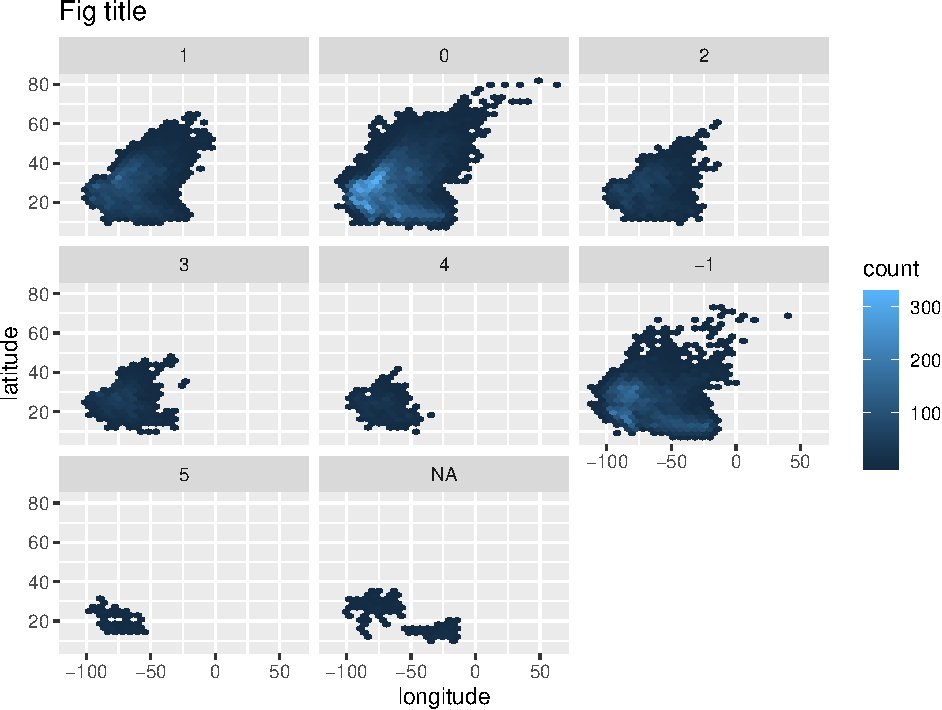
\includegraphics[width=0.8\linewidth]{edav-final-project_files/figure-latex/hex-fig-1} 

}

\caption{Here is a nice figure!}\label{fig:hex-fig}
\end{figure}

\begin{Shaded}
\begin{Highlighting}[]
\CommentTok{# need to add map}
\end{Highlighting}
\end{Shaded}

Figure \ref{fig:hex-fig} shows

\begin{Shaded}
\begin{Highlighting}[]
\KeywordTok{library}\NormalTok{(gridExtra)}

\NormalTok{df }\OperatorTok
\StringTok{        }\KeywordTok{ggplot}\NormalTok{()}\OperatorTok{+}
\StringTok{        }\KeywordTok{geom_boxplot}\NormalTok{(}\KeywordTok{aes}\NormalTok{(}\DataTypeTok{x=}\KeywordTok{reorder}\NormalTok{(category, max_wind, median), }\DataTypeTok{y=}\NormalTok{latitude), }\DataTypeTok{varwidth =} \OtherTok{TRUE}\NormalTok{)}\OperatorTok{+}
\StringTok{        }\CommentTok{#coord_flip()}
\StringTok{        }\KeywordTok{facet_wrap}\NormalTok{(}\OperatorTok{~}\NormalTok{status, }\DataTypeTok{scale=}\StringTok{"free"}\NormalTok{)}
\end{Highlighting}
\end{Shaded}

\begin{figure}

{\centering 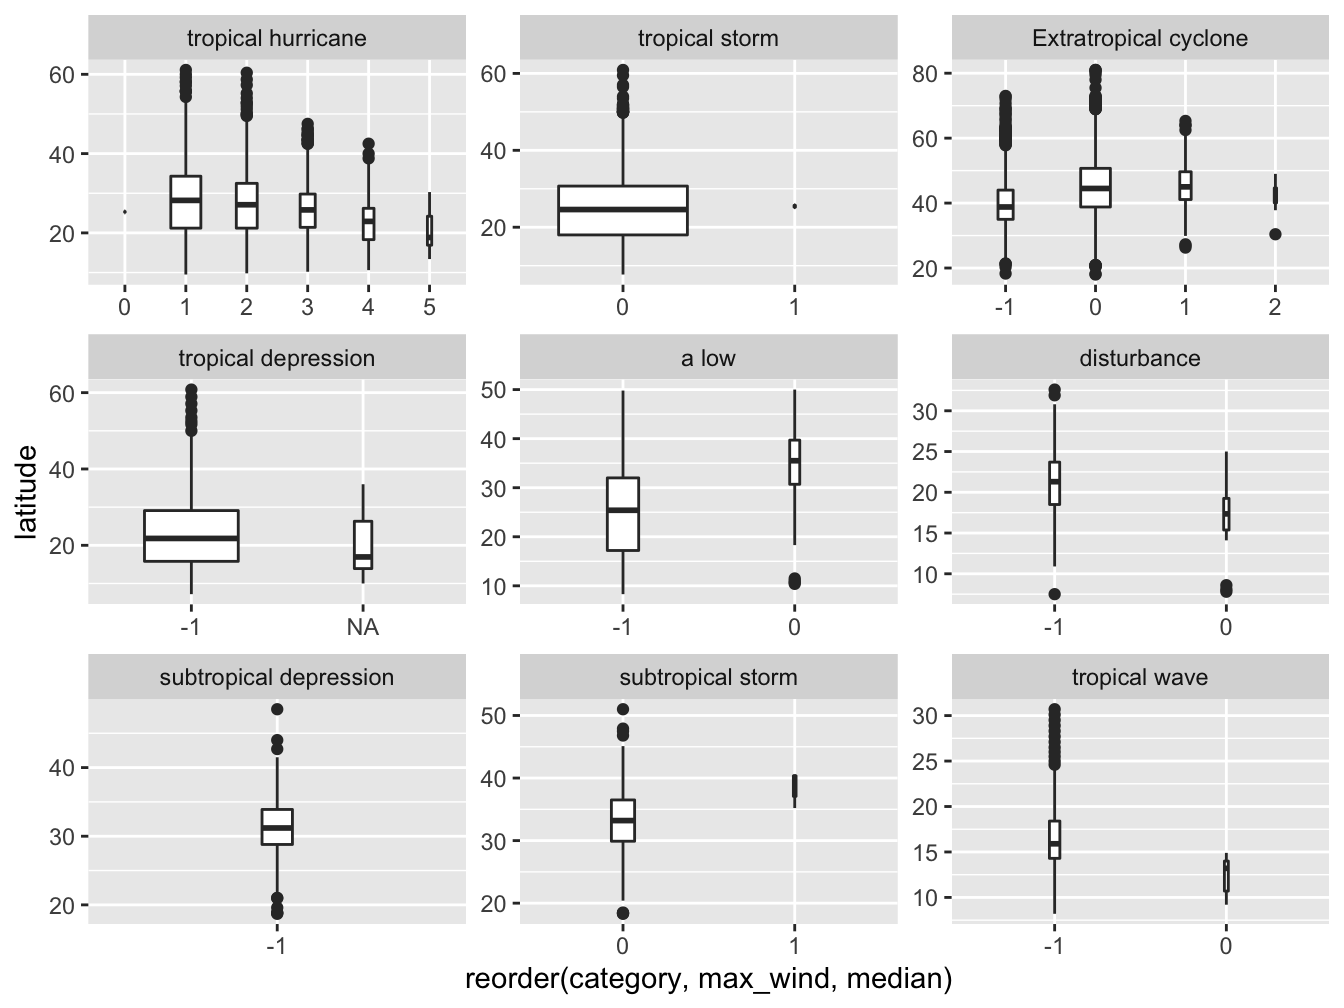
\includegraphics[width=0.8\linewidth]{edav-final-project_files/figure-latex/boxplot-wind-category-lat-fig-1} 

}

\caption{Here is a nice figure!}\label{fig:boxplot-wind-category-lat-fig}
\end{figure}

\begin{Shaded}
\begin{Highlighting}[]
\KeywordTok{library}\NormalTok{(gridExtra)}

\NormalTok{df }\OperatorTok
\StringTok{        }\KeywordTok{ggplot}\NormalTok{()}\OperatorTok{+}
\StringTok{        }\KeywordTok{geom_boxplot}\NormalTok{(}\KeywordTok{aes}\NormalTok{(}\DataTypeTok{x=}\KeywordTok{reorder}\NormalTok{(category, max_wind, median), }\DataTypeTok{y=}\NormalTok{hu_diameter), }\DataTypeTok{varwidth =} \OtherTok{TRUE}\NormalTok{)}\OperatorTok{+}
\StringTok{        }\CommentTok{#coord_flip()}
\StringTok{        }\CommentTok{#facet_wrap(~status)#, scale="free")+}
\StringTok{        }\KeywordTok{labs}\NormalTok{(}\DataTypeTok{title =} \StringTok{"Fig title"}\NormalTok{)}
\end{Highlighting}
\end{Shaded}

\begin{figure}

{\centering 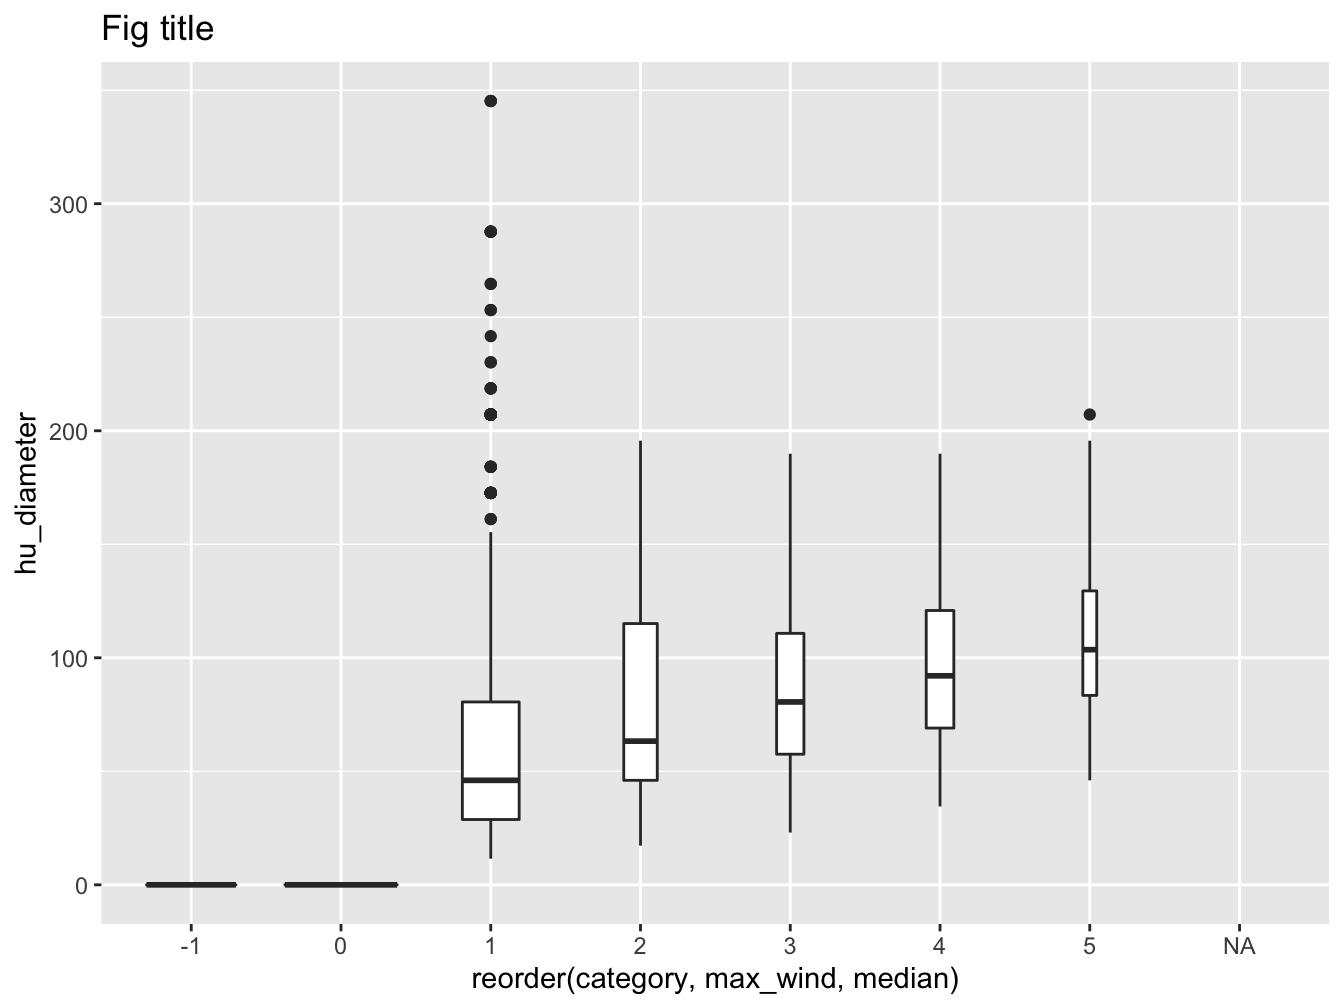
\includegraphics[width=0.8\linewidth]{edav-final-project_files/figure-latex/boxplot-wind-category-hu-fig-1} 

}

\caption{Here is a nice figure!}\label{fig:boxplot-wind-category-hu-fig}
\end{figure}

\begin{Shaded}
\begin{Highlighting}[]
\KeywordTok{library}\NormalTok{(ggridges)}
\KeywordTok{library}\NormalTok{(viridis)}
\NormalTok{df }\OperatorTok
\StringTok{        }\KeywordTok{ggplot}\NormalTok{()}\OperatorTok{+}
\StringTok{        }\KeywordTok{geom_density_ridges_gradient}\NormalTok{(}\KeywordTok{aes}\NormalTok{(}\DataTypeTok{x=}\NormalTok{ year, }\DataTypeTok{y=}\NormalTok{ category, }\DataTypeTok{group =}\NormalTok{ category, }\DataTypeTok{fill =}\NormalTok{ ..x.., }\DataTypeTok{scale =} \FloatTok{0.9}\NormalTok{))}\OperatorTok{+}
\StringTok{        }\KeywordTok{scale_fill_viridis}\NormalTok{()}\OperatorTok{+}
\StringTok{        }\CommentTok{#coord_flip()+}
\StringTok{        }\KeywordTok{labs}\NormalTok{(}\DataTypeTok{title =} \StringTok{"Fig title"}\NormalTok{)}
\end{Highlighting}
\end{Shaded}

\begin{figure}

{\centering 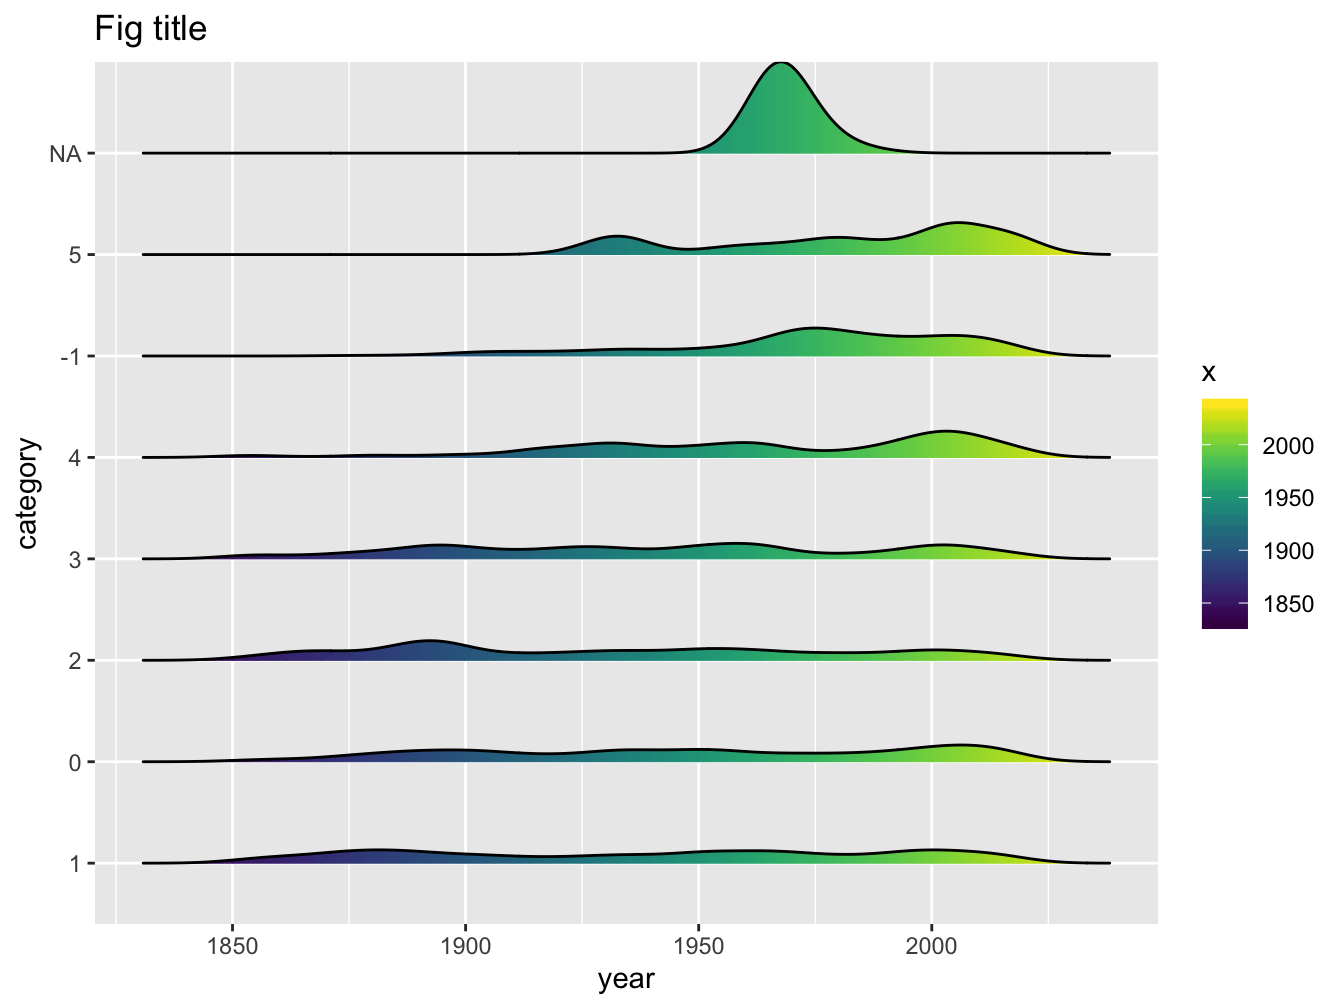
\includegraphics[width=0.8\linewidth]{edav-final-project_files/figure-latex/ridges-year-category-fig-1} 

}

\caption{Here is a nice figure!}\label{fig:ridges-year-category-fig}
\end{figure}

\begin{Shaded}
\begin{Highlighting}[]
\KeywordTok{library}\NormalTok{(ggridges)}
\KeywordTok{library}\NormalTok{(viridis)}
\NormalTok{df }\OperatorTok
\StringTok{        }\KeywordTok{ggplot}\NormalTok{()}\OperatorTok{+}
\StringTok{        }\KeywordTok{geom_density_ridges_gradient}\NormalTok{(}\KeywordTok{aes}\NormalTok{(}\DataTypeTok{x=}\NormalTok{ year, }\DataTypeTok{y=}\NormalTok{ status, }\DataTypeTok{group =}\NormalTok{ status, }\DataTypeTok{fill =}\NormalTok{ ..x.., }\DataTypeTok{scale =} \FloatTok{0.9}\NormalTok{))}\OperatorTok{+}
\StringTok{        }\KeywordTok{scale_fill_viridis}\NormalTok{()}\OperatorTok{+}
\StringTok{        }\CommentTok{#coord_flip()+}
\StringTok{        }\CommentTok{#facet_wrap(~cluster_name_more_short, scale="free", ncol = 1)+}
\StringTok{        }\KeywordTok{labs}\NormalTok{(}\DataTypeTok{title =} \StringTok{"Fig title"}\NormalTok{)}
\end{Highlighting}
\end{Shaded}

\begin{figure}

{\centering 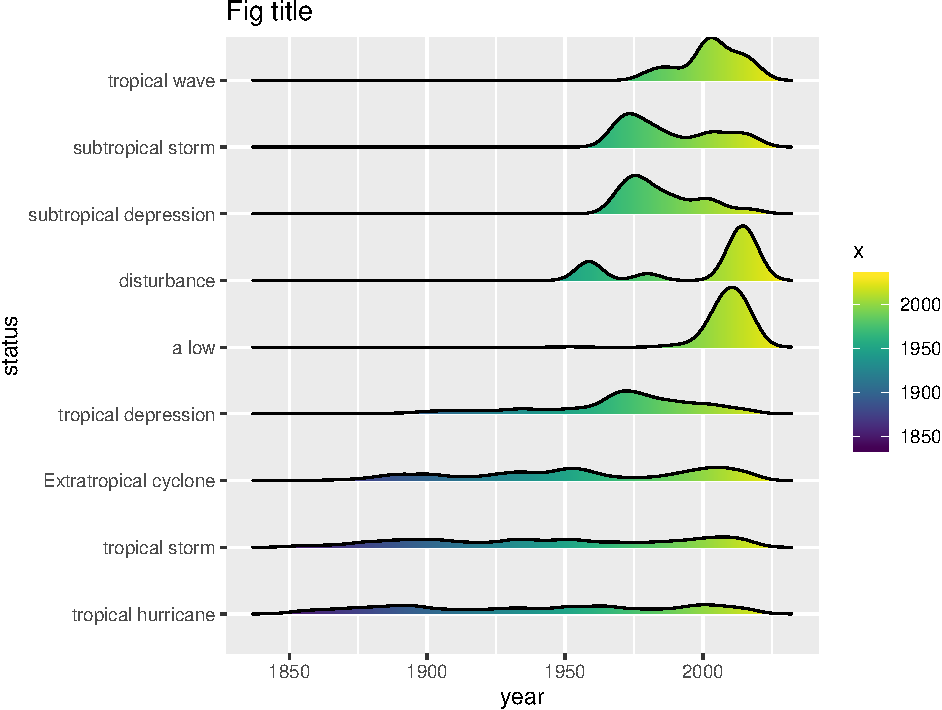
\includegraphics[width=0.8\linewidth]{edav-final-project_files/figure-latex/density-year-status-fig-1} 

}

\caption{Here is a nice figure!}\label{fig:density-year-status-fig}
\end{figure}

\begin{Shaded}
\begin{Highlighting}[]
\CommentTok{# cleveland}
\end{Highlighting}
\end{Shaded}

\begin{Shaded}
\begin{Highlighting}[]
\KeywordTok{library}\NormalTok{(parcoords)}

\CommentTok{#df %>%}
\CommentTok{#        dplyr::select( ts_diameter, hu_diameter, min_pressure, max_wind, category, status) %>% }
\CommentTok{#  drop_na() %>% }
\CommentTok{#        parcoords(alpha = 0.2,}
\CommentTok{#                  color = list(colorBy = "category"),}
\CommentTok{#                  withD3 = TRUE,}
\CommentTok{#                  rownames = FALSE,}
\CommentTok{#                  reorderable = TRUE,}
\CommentTok{#                  brushMode = "1d-axes")}
\end{Highlighting}
\end{Shaded}

\begin{Shaded}
\begin{Highlighting}[]
\NormalTok{df }\OperatorTok
\StringTok{  }\KeywordTok{drop_na}\NormalTok{() }\OperatorTok\StringTok{ }\KeywordTok{filter}\NormalTok{(name }\OperatorTok{==}\StringTok{"Katrina"}\NormalTok{) }\OperatorTok\StringTok{ }
\StringTok{  }\KeywordTok{ggplot}\NormalTok{(}\KeywordTok{aes}\NormalTok{(}\DataTypeTok{x=}\NormalTok{longitude, }\DataTypeTok{y=}\NormalTok{latitude, }\DataTypeTok{color=}\NormalTok{ts_diameter))}\OperatorTok{+}
\StringTok{  }\KeywordTok{geom_point}\NormalTok{()}
\end{Highlighting}
\end{Shaded}

\begin{figure}

{\centering 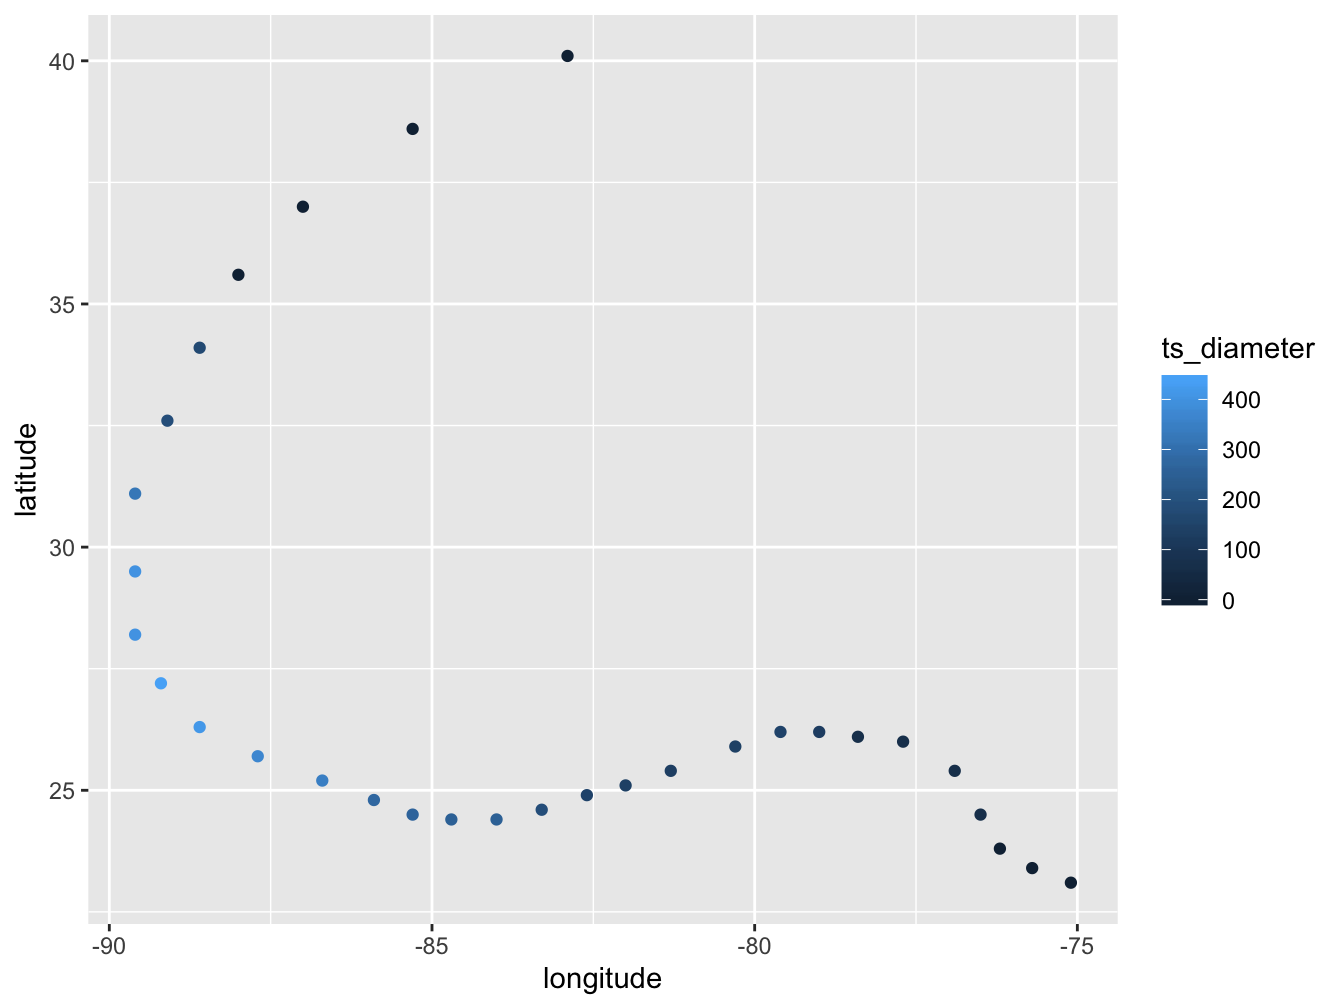
\includegraphics[width=0.8\linewidth]{edav-final-project_files/figure-latex/point-date-wind-fig-1} 

}

\caption{Here is a nice figure!}\label{fig:point-date-wind-fig1}
\end{figure}

\begin{Shaded}
\begin{Highlighting}[]
\CommentTok{## need to add map}

\NormalTok{df }\OperatorTok
\StringTok{  }\KeywordTok{drop_na}\NormalTok{() }\OperatorTok\StringTok{ }\KeywordTok{filter}\NormalTok{(name }\OperatorTok{==}\StringTok{"Katrina"}\NormalTok{) }\OperatorTok\StringTok{ }
\StringTok{  }\KeywordTok{ggplot}\NormalTok{(}\KeywordTok{aes}\NormalTok{(}\DataTypeTok{x=}\NormalTok{datetime, }\DataTypeTok{y=}\NormalTok{max_wind, }\DataTypeTok{color=}\NormalTok{category))}\OperatorTok{+}
\StringTok{  }\KeywordTok{geom_point}\NormalTok{()}
\end{Highlighting}
\end{Shaded}

\begin{figure}

{\centering 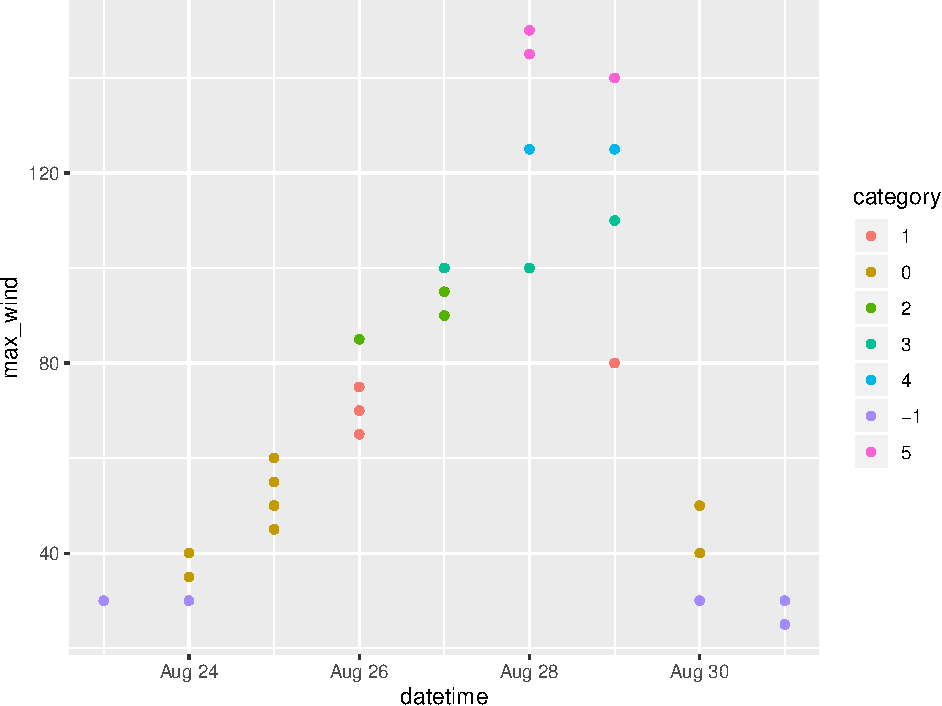
\includegraphics[width=0.8\linewidth]{edav-final-project_files/figure-latex/point-date-wind-fig-2} 

}

\caption{Here is a nice figure!}\label{fig:point-date-wind-fig2}
\end{figure}

\begin{Shaded}
\begin{Highlighting}[]
\KeywordTok{library}\NormalTok{(plotly)}
\CommentTok{#df %>%}
\CommentTok{#  drop_na() %>% }
\CommentTok{#  filter(name =="Katrina") %>%}
\CommentTok{#  plot_ly(x=~datetime, y=~max_wind)}
\end{Highlighting}
\end{Shaded}

\begin{Shaded}
\begin{Highlighting}[]
\KeywordTok{levels}\NormalTok{(df }\OperatorTok\StringTok{ }\KeywordTok{filter}\NormalTok{(completeish}\OperatorTok{==}\StringTok{"yes"}\NormalTok{) }\OperatorTok\StringTok{ }\NormalTok{.}\OperatorTok{$}\NormalTok{status)}
\end{Highlighting}
\end{Shaded}

\begin{verbatim}
## [1] "tropical hurricane"     "tropical storm"         "Extratropical cyclone" 
## [4] "tropical depression"    "a low"                  "disturbance"           
## [7] "subtropical depression" "subtropical storm"      "tropical wave"
\end{verbatim}

\begin{Shaded}
\begin{Highlighting}[]
\CommentTok{#names(df)}
\NormalTok{df_selected <-}\StringTok{ }\NormalTok{df }\OperatorTok\StringTok{ }
\StringTok{  }\CommentTok{#filter(completeish == "yes") %>% }
\StringTok{  }\KeywordTok{filter}\NormalTok{(year}\OperatorTok{>}\DecValTok{1990}\NormalTok{) }\OperatorTok\StringTok{ }
\StringTok{  }\CommentTok{#filter (status == c("hurricane","tropical storm","tropical depression")) %>%}
\StringTok{  }\KeywordTok{filter}\NormalTok{(hu_diameter}\OperatorTok{>}\DecValTok{0}\NormalTok{) }\OperatorTok\StringTok{ }
\StringTok{  }\KeywordTok{drop_na}\NormalTok{() }\OperatorTok\StringTok{ }
\StringTok{  }\NormalTok{dplyr}\OperatorTok{::}\KeywordTok{mutate}\NormalTok{(}\DataTypeTok{decade=}\KeywordTok{cut}\NormalTok{(year,}
                           \DataTypeTok{breaks =} \KeywordTok{c}\NormalTok{(}\DecValTok{2000}\NormalTok{, }\DecValTok{2005}\NormalTok{, }\DecValTok{2010}\NormalTok{, }\DecValTok{2015}\NormalTok{, }\DecValTok{2020}\NormalTok{),}
                           \DataTypeTok{lables =} \KeywordTok{c}\NormalTok{(}\StringTok{'00s'}\NormalTok{, }\StringTok{'05s'}\NormalTok{,}\StringTok{'10s'}\NormalTok{,}\StringTok{'15'}\NormalTok{, }\StringTok{'20s'}\NormalTok{),}
                           \DataTypeTok{include.lowest =} \OtherTok{TRUE}\NormalTok{, }\DataTypeTok{ordered=}\OtherTok{TRUE}\NormalTok{))}
\end{Highlighting}
\end{Shaded}

\begin{Shaded}
\begin{Highlighting}[]
\KeywordTok{library}\NormalTok{(ggmosaic)}
\KeywordTok{ggplot}\NormalTok{(}\DataTypeTok{data =}\NormalTok{ df_selected) }\OperatorTok{+}
\StringTok{   }\KeywordTok{geom_mosaic}\NormalTok{(}\KeywordTok{aes}\NormalTok{(}\DataTypeTok{x =} \KeywordTok{product}\NormalTok{(category, decade), }\DataTypeTok{fill=}\NormalTok{category), }\DataTypeTok{na.rm=}\OtherTok{TRUE}\NormalTok{)}
\end{Highlighting}
\end{Shaded}

\begin{figure}

{\centering 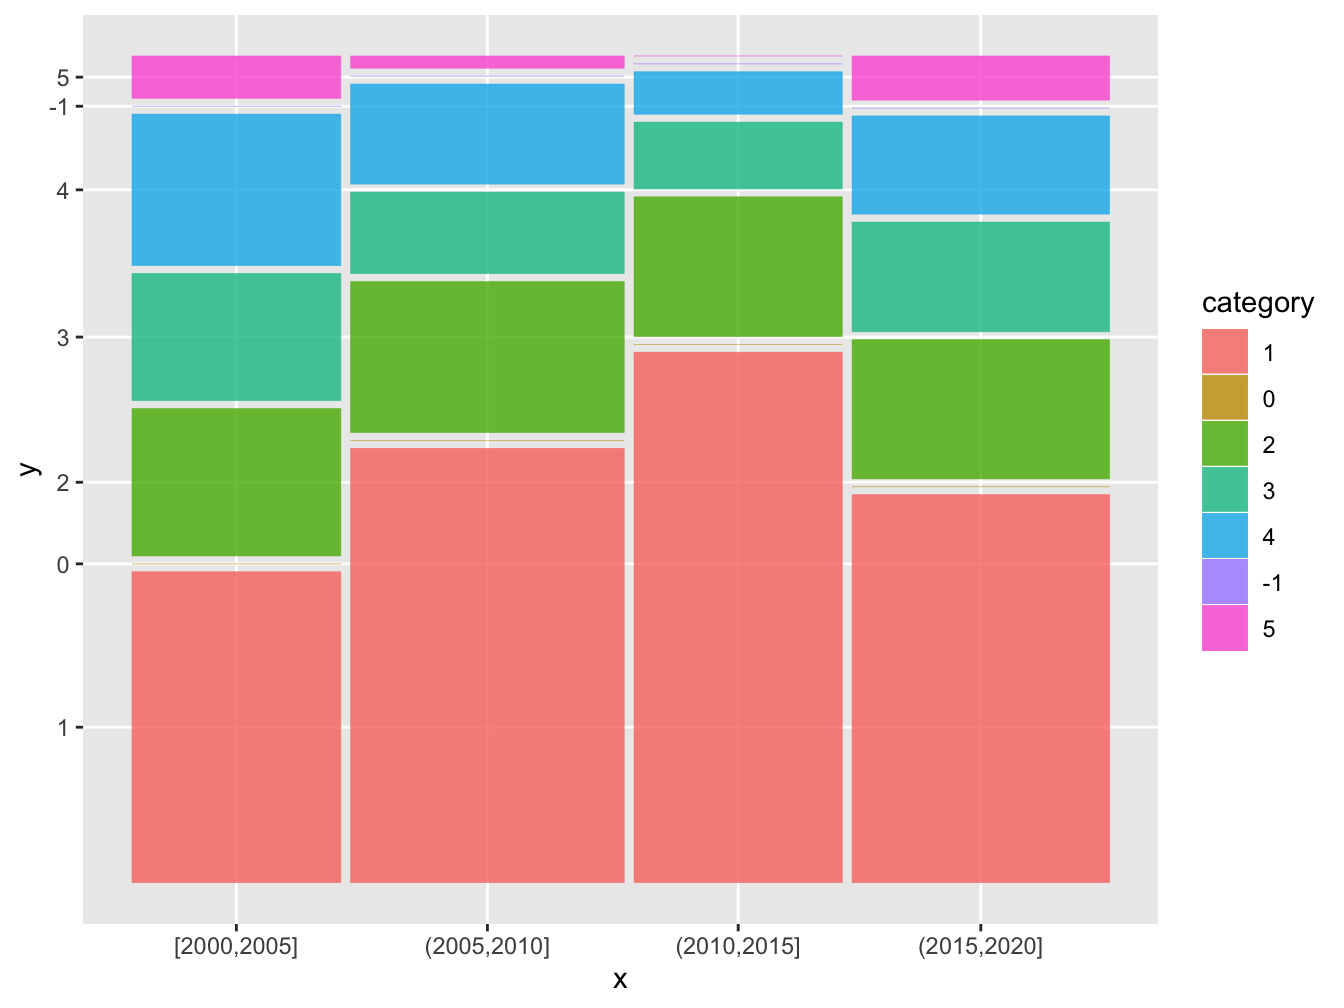
\includegraphics[width=0.8\linewidth]{edav-final-project_files/figure-latex/mosaic-hdecade-category-fig-1} 

}

\caption{Here is a nice figure!}\label{fig:mosaic-hdecade-category-fig}
\end{figure}

\begin{Shaded}
\begin{Highlighting}[]
\KeywordTok{library}\NormalTok{(ggmosaic)}
\KeywordTok{ggplot}\NormalTok{(}\DataTypeTok{data =}\NormalTok{ df_selected) }\OperatorTok{+}
\StringTok{   }\KeywordTok{geom_mosaic}\NormalTok{(}\KeywordTok{aes}\NormalTok{(}\DataTypeTok{x =} \KeywordTok{product}\NormalTok{(category, month), }\DataTypeTok{fill=}\NormalTok{category), }\DataTypeTok{na.rm=}\OtherTok{TRUE}\NormalTok{)}
\end{Highlighting}
\end{Shaded}

\begin{figure}

{\centering 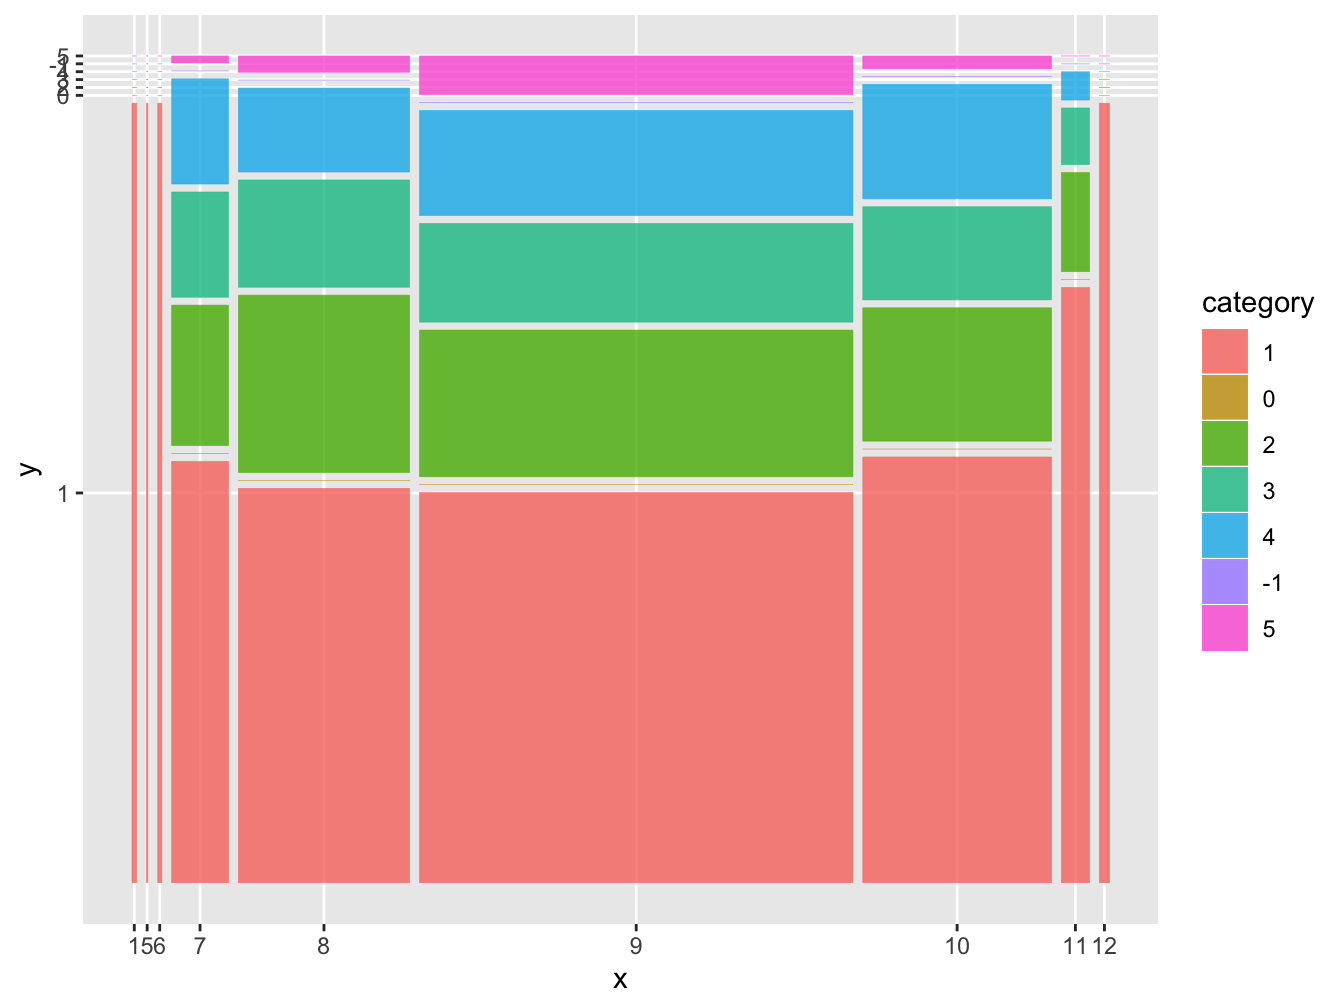
\includegraphics[width=0.8\linewidth]{edav-final-project_files/figure-latex/mosaic-category-month-fig-1} 

}

\caption{Here is a nice figure!}\label{fig:mosaic-category-month-fig}
\end{figure}

\begin{Shaded}
\begin{Highlighting}[]
\NormalTok{df }\OperatorTok
\StringTok{  }\KeywordTok{select}\NormalTok{(}\KeywordTok{c}\NormalTok{(}\StringTok{"year"}\NormalTok{, }\StringTok{"id"}\NormalTok{, }\StringTok{"status"}\NormalTok{)) }\OperatorTok\StringTok{ }
\StringTok{  }\KeywordTok{unique}\NormalTok{() }\OperatorTok\StringTok{ }
\StringTok{  }\KeywordTok{group_by}\NormalTok{(year, status) }\OperatorTok\StringTok{ }
\StringTok{  }\KeywordTok{drop_na}\NormalTok{() }\OperatorTok\StringTok{ }
\StringTok{  }\KeywordTok{count}\NormalTok{() }\OperatorTok\StringTok{ }
\StringTok{  }\KeywordTok{ungroup}\NormalTok{() }\OperatorTok\StringTok{ }
\StringTok{  }\KeywordTok{ggplot}\NormalTok{(}\KeywordTok{aes}\NormalTok{(}\DataTypeTok{x=}\NormalTok{year, }\DataTypeTok{y=}\NormalTok{n))}\OperatorTok{+}
\StringTok{  }\KeywordTok{geom_line}\NormalTok{()}\OperatorTok{+}
\StringTok{  }\KeywordTok{facet_wrap}\NormalTok{(}\OperatorTok{~}\NormalTok{status, }\DataTypeTok{scale=}\StringTok{"free"}\NormalTok{)}
\end{Highlighting}
\end{Shaded}

\begin{figure}

{\centering 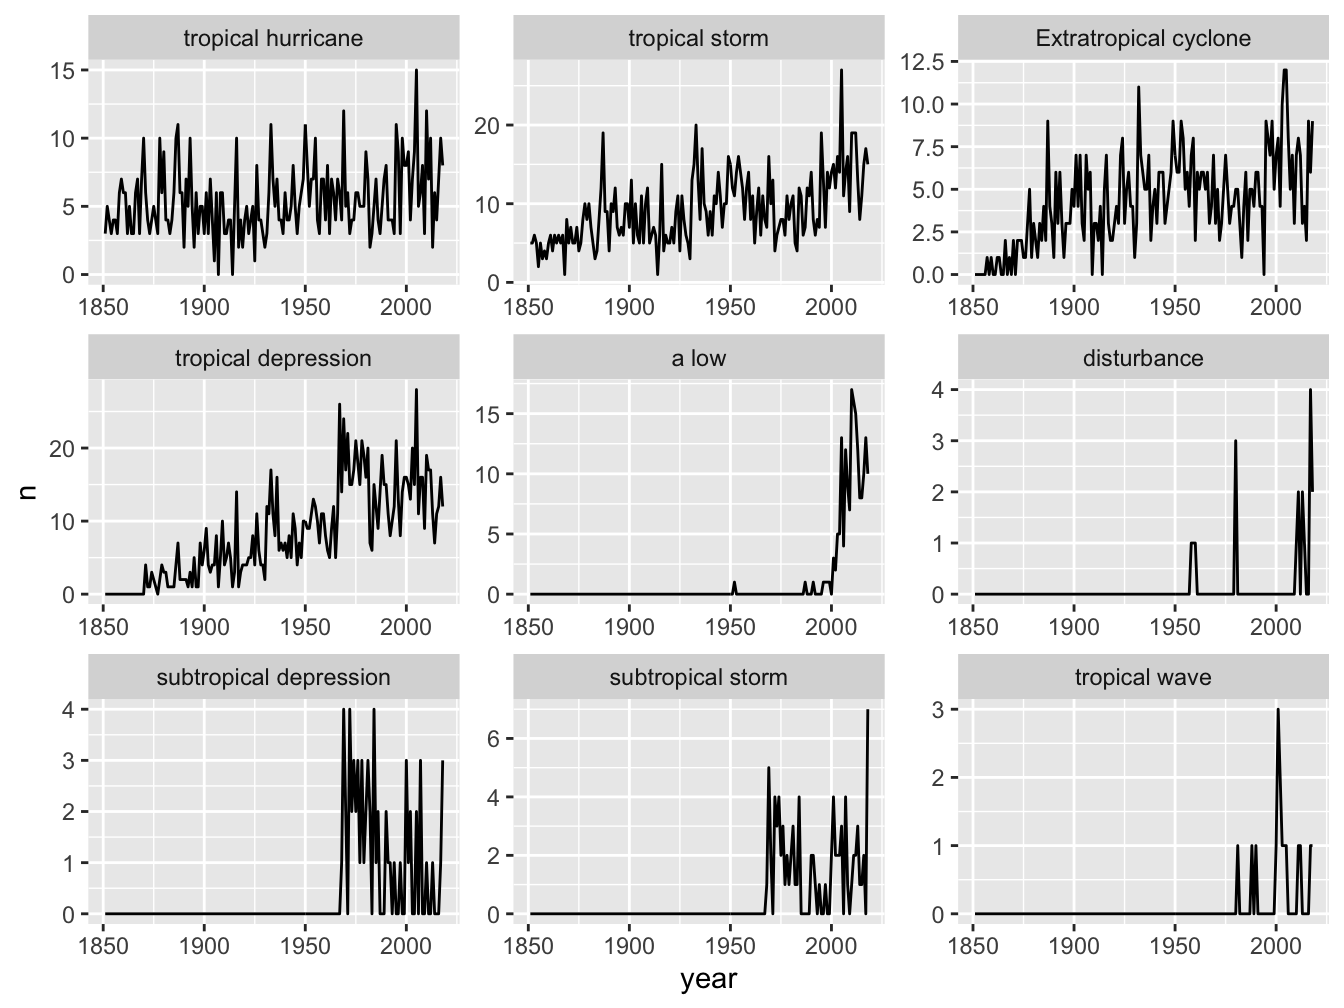
\includegraphics[width=0.8\linewidth]{edav-final-project_files/figure-latex/year-count-fig-1} 

}

\caption{Here is a nice figure!}\label{fig:year-count-fig}
\end{figure}

\hypertarget{tables}{%
\section{Tables}\label{tables}}

Summary table if applicable

We can reference tables generated from \texttt{knitr::kable()}, e.g., see Table \ref{tab:nice-tab}.
And it works even the item is not in this chapter.

\begin{Shaded}
\begin{Highlighting}[]
\NormalTok{knitr}\OperatorTok{::}\KeywordTok{kable}\NormalTok{(}
  \KeywordTok{head}\NormalTok{(df_selected[}\DecValTok{2}\OperatorTok{:}\DecValTok{3}\NormalTok{], }\DecValTok{10}\NormalTok{), }\DataTypeTok{caption =} \StringTok{'Here is a nice table!'}\NormalTok{,}
  \DataTypeTok{booktabs =} \OtherTok{TRUE}
\NormalTok{)}
\end{Highlighting}
\end{Shaded}

\begin{table}

\caption{\label{tab:nice-tab}Here is a nice table!}
\centering
\begin{tabular}[t]{ll}
\toprule
name & datetime\\
\midrule
Alex & 2004-08-03\\
Alex & 2004-08-03\\
Alex & 2004-08-03\\
Alex & 2004-08-04\\
Alex & 2004-08-04\\
\addlinespace
Alex & 2004-08-04\\
Alex & 2004-08-04\\
Alex & 2004-08-05\\
Alex & 2004-08-05\\
Alex & 2004-08-05\\
\bottomrule
\end{tabular}
\end{table}

\hypertarget{interactive-component}{%
\chapter{Interactive Component}\label{interactive-component}}

Select one (or more) of our key findings to present in an interactive format (D3). Be selective in the choices that we present to the user; the idea is that in 5-10 minutes, users should have a good sense of the question(s) that we are interested in and the trends we've identified in the data. In other words, they should understand the value of the analysis, be it business value, scientific value, general knowledge, etc.

\hypertarget{conclusion}{%
\chapter{Conclusion}\label{conclusion}}

Discuss limitations and future directions, lessons learned.

\bibliography{proj.bib,packages.bib}


\end{document}
